\documentclass[11pt]{article}
\usepackage[margin=1in]{geometry}
\usepackage{amsmath,amssymb,amsfonts}
\usepackage{graphicx}
\usepackage{booktabs}
\usepackage[hidelinks]{hyperref}
\usepackage{placeins}
\usepackage{float}
\usepackage{natbib}
\usepackage{algorithm}
\usepackage{algorithmic}

\title{AD-IRT: Adaptive Dimensionality Item Response Theory\\for Sparse Cross-Benchmark Evaluation}

\author{Jung Min Kang\\Independent Researcher\\Seoul, South Korea\\{\tt gangjeongmin23@gmail.com}\\ORCID: 0009-0007-9599-2792}

\date{May 2026}

\begin{document}
\maketitle

\begin{abstract}
Item Response Theory (IRT) corrects the ranking failures of simple benchmark averaging under sparse evaluation conditions~\citep{kang2026efsl}, but assumes a single latent ability dimension. Multidimensional IRT (MIRT) captures richer structure but requires more parameters and data to converge. We introduce \textbf{AD-IRT} (Adaptive Dimensionality IRT), which blends IRT and MIRT predictions per model using a coverage-breadth-modulated weight. On public Evo-SOTA.io VLA benchmark data (147 models, 29 items across 7 benchmark families, 20.3\% coverage), nested 5-fold cross-validation---where the blend parameter $w$ is tuned on inner folds and evaluated on held-out outer folds---shows AD-IRT achieves $\rho = 0.851 \pm 0.023$, outperforming both IRT ($\rho = 0.839 \pm 0.021$) and simple averaging ($\rho = 0.799 \pm 0.029$). AD-IRT wins in 4 of 5 folds with mean $\Delta\rho = +0.013$. Standard errors use sample SEM ($\mathrm{ddof}=1$, $n=5$ folds). Model family count $f_u$ is computed from the full observation mask (not from training data alone), treating reporting breadth as known metadata rather than a quantity to be estimated. A sensitivity analysis computing $f_u$ from training-only observations yields $\rho = 0.845 \pm 0.021$ (vs.\ $0.851 \pm 0.023$), showing a weaker but directionally consistent effect; 80\% subsampling rarely removes a model's only observation in a family. Empirically, the learned blend assigns more MIRT weight to narrow-coverage models, suggesting that MIRT contributes primarily through item-side cross-family difficulty calibration rather than model-side multidimensional ability estimation.
\end{abstract}

\noindent\textbf{Keywords:} Item Response Theory, MIRT, Physical AI, adaptive model selection, VLA benchmarks

\section{Introduction}

Vision-language-action (VLA) model evaluation suffers from extreme fragmentation. Public leaderboards such as Evo-SOTA.io~\citep{evosota2026} aggregate results across LIBERO~\citep{liu2023libero}, CALVIN~\citep{mees2022calvin}, Meta-World~\citep{yu2020metaworld}, LIBERO-Plus~\citep{fei2025liberoplus}, and dexterous manipulation benchmarks, but most models report on only a subset. The resulting score matrix has 20.3\% coverage---the sparse regime where simple averaging produces misleading rankings~\citep{kang2026efsl}.

The Evaluation Failure Scaling Law (EFSL) established that IRT maintains ranking accuracy ($\rho \geq 0.993$) across all sparsity and difficulty conditions where simple averaging degrades to $\rho = 0.24$~\citep{kang2026efsl}. However, standard 1PL IRT assumes a single latent ability dimension. When benchmark items span multiple skill dimensions---manipulation, robustness, long-horizon planning, dexterous control---a unidimensional model may lose information.

Multidimensional IRT (MIRT;~\citealt{reckase2009}) addresses this by estimating $K$-dimensional ability vectors. Recent work showed that 3D MIRT outperforms matrix factorization up to 20 dimensions on MovieLens-1M~\citep{veldkamp2025}. However, MIRT requires substantially more parameters, and on sparse evaluation matrices, this becomes a liability.

We observe that the optimal model complexity varies \emph{within} the same evaluation matrix: 59\% of VLA models report on only one benchmark family (typically LIBERO's four suites), while 8\% report across three or more families. A single model complexity cannot serve both groups optimally.

\paragraph{Contribution.} We introduce AD-IRT (Adaptive Dimensionality IRT), which:
\begin{enumerate}
    \item Fits both 1PL IRT and MIRT on the same training data;
    \item Blends their predictions per model via $\alpha_u = \sigma(w \cdot (f_u - c))$, where $f_u$ is the number of benchmark families model $u$ reports on;
    \item Learns $w$ via inner cross-validation (no test leakage).
\end{enumerate}

On nested 5-fold CV over real Evo-SOTA.io data, AD-IRT achieves $\rho = 0.851 \pm 0.023$, outperforming IRT ($0.839$), MIRT ($0.775$), and simple averaging ($0.799$) in 4 of 5 folds.

\section{Background}

\subsection{1PL IRT for Benchmark Evaluation}

We use a Rasch-style fractional logistic model inspired by 1PL IRT~\citep{lord1968}. For model $i$ and item $j$, the expected normalized success score is:
\begin{equation}
\mathbb{E}[s_{ij} \mid \theta_i, b_j] = \sigma(\theta_i - b_j)
\label{eq:irt}
\end{equation}
where $\theta_i \in \mathbb{R}$ is latent ability and $b_j \in \mathbb{R}$ is item difficulty. IRT jointly estimates $\theta$ and $b$ from observed data, automatically adjusting for the difficulty of each model's evaluation items~\citep{kang2026efsl, rodriguez2021}.

\subsection{Multidimensional IRT}

MIRT~\citep{reckase2009} extends IRT to $K$ latent dimensions:
\begin{equation}
\mathbb{E}[s_{ij} \mid \boldsymbol{\theta}_i, \mathbf{a}_j, d_j] = \sigma(\mathbf{a}_j^\top \boldsymbol{\theta}_i + d_j)
\label{eq:mirt}
\end{equation}
where $\boldsymbol{\theta}_i \in \mathbb{R}^K$, $\mathbf{a}_j \in \mathbb{R}^K$, and $d_j \in \mathbb{R}$. MIRT requires $K(N + M) + M$ parameters versus $N + M$ for 1PL.

\subsection{The Data Regime Problem}

For our VLA data with $O = 864$ observations: 1PL has $O/P = 864/176 = 4.9$; MIRT $K\!=\!2$ has $O/P = 864/381 = 2.3$. Individual models with broad coverage effectively have higher per-model $O/P$, while narrow-coverage models have lower---motivating a per-model adaptive approach.

\section{AD-IRT: Adaptive Dimensionality IRT}

\begin{algorithm}[t]
\caption{AD-IRT: Adaptive Dimensionality IRT}
\begin{algorithmic}[1]
\REQUIRE Training score matrix $\mathbf{S}_{\mathrm{train}}$, family mapping $\mathcal{F}$, center $c$
\STATE Fit 1PL IRT on $\mathbf{S}_{\mathrm{train}}$ $\rightarrow$ $\{\theta_i, b_j\}$
\STATE Fit MIRT($K$) on $\mathbf{S}_{\mathrm{train}}$ $\rightarrow$ $\{\boldsymbol{\theta}_i, \mathbf{a}_j, d_j\}$
\STATE $f_u \leftarrow$ number of families model $u$ reports on
\STATE Select $w^*$ via inner cross-validation on training data
\FOR{each (model $u$, item $j$)}
    \STATE $\alpha_u \leftarrow \sigma(w^* \cdot (f_u - c))$
    \STATE $\hat{p}_{uj} \leftarrow (1 - \alpha_u) \cdot \sigma(\theta_u - b_j) + \alpha_u \cdot \sigma(\mathbf{a}_j^\top \boldsymbol{\theta}_u + d_j)$
\ENDFOR
\end{algorithmic}
\end{algorithm}

AD-IRT blends IRT and MIRT predictions:
\begin{equation}
\hat{p}_{uj} = (1 - \alpha_u) \cdot P_{\text{IRT}}(u,j) + \alpha_u \cdot P_{\text{MIRT}}(u,j)
\label{eq:adirt}
\end{equation}
where $\alpha_u = \sigma(w \cdot (f_u - c))$ and $f_u$ is the number of benchmark families model $u$ reports on. The single scalar $w$ is selected via 3-fold inner CV within each outer training fold.

\paragraph{Computational cost.} AD-IRT adds one sigmoid evaluation per prediction beyond the combined cost of fitting IRT and MIRT. The $w$ grid search is one-dimensional and adds negligible cost.

\section{Experimental Setup}

\subsection{Data}

We parse public JSON data from Evo-SOTA.io~\citep{evosota2026} for seven benchmark families: LIBERO (4 suites), LIBERO-Plus (7 perturbation types), CALVIN (3 splits), Meta-World (4 difficulty levels), Dexterous manipulation (7 tasks across Adroit and DexArt), RoboTwin (2 difficulty levels), and RoboCasa/RoboChallenge. After filtering to models with $\geq$3 items and items with $\geq$5 models, the matrix contains 147 models $\times$ 29 items with 864 observed scores (20.3\% coverage). Table~\ref{tab:items} shows the item structure.

\begin{table}[htbp]
\centering
\caption{Benchmark items by family with reporting coverage.}
\label{tab:items}
\small
\begin{tabular}{llr}
\toprule
Family & Items & Coverage \\
\midrule
LIBERO (4) & Spatial, Object, Goal, Long & 82--83\% \\
LIBERO-Plus (7) & Background, Camera, Language, Layout, Light, Noise, Robot & 17\% \\
CALVIN (3) & ABC, ABCD, D & 5--14\% \\
Meta-World (4) & Easy, Medium, Hard, Very-Hard & 5--8\% \\
Dexterous (7) & Adroit \{pen, door, hammer\}, DexArt \{laptop, faucet, toilet, bucket\} & 7--8\% \\
RoboTwin (2) & Easy, Hard & 9\% \\
Other (2) & RoboCasa, RoboChallenge & 4--5\% \\
\bottomrule
\end{tabular}
\end{table}

\subsection{Evaluation Protocol}

We use \textbf{nested 5-fold cross-validation} to prevent test leakage. In each outer fold: (1)~the training set is further split into 3 inner folds; (2)~for each candidate $w \in \{-3.0, -2.5, \ldots, +3.5\}$, IRT and MIRT are fitted on inner training data, and blended predictions are evaluated on inner validation data; (3)~the $w$ with highest inner-CV ranking correlation is selected; (4)~IRT and MIRT are refit on the full outer training set; (5)~predictions are evaluated on the outer test set using the frozen $w$. The primary metric is Spearman $\rho$ between predicted and actual model-level mean scores on held-out data.

\FloatBarrier
\section{Results}

\subsection{Nested Cross-Validation}

Table~\ref{tab:cv} presents the main results. AD-IRT achieves the highest ranking correlation, winning 4 of 5 folds.

\begin{table}[htbp]
\centering
\caption{Nested 5-fold CV results (mean $\pm$ SEM). $w$ is tuned on inner folds and frozen for outer evaluation. AD-IRT wins 4/5 folds with mean $\Delta\rho = +0.013$ over IRT.}
\label{tab:cv}
\begin{tabular}{lcccc}
\toprule
Method & Rank $\rho$ & MAE & Wins & $\Delta\rho$ vs IRT \\
\midrule
Simple Averaging & $0.799 \pm 0.029$ & $\mathbf{0.106 \pm 0.002}$ & 0/5 & $-0.040$ \\
IRT 1PL & $0.839 \pm 0.021$ & $0.205 \pm 0.006$ & --- & --- \\
MIRT $K\!=\!2$ & $0.775 \pm 0.035$ & $0.287 \pm 0.006$ & 1/5 & $-0.064$ \\
\textbf{AD-IRT} & $\mathbf{0.851 \pm 0.023}$ & $0.244 \pm 0.006$ & \textbf{4/5} & $+0.013$ \\
\bottomrule
\end{tabular}
\end{table}

The inner-CV-selected $w$ values are $\{-0.5, -0.5, -0.5, -0.5, -0.5\}$ across all five outer folds ($\bar{w} = -0.50$), showing stable selection of negative $w$. The Wilcoxon signed-rank test for AD-IRT $>$ IRT gives $p = 0.0625$, marginal at $\alpha = 0.05$ due to the small number of folds but consistent in direction.

\subsection{Coverage--Difficulty Correlation}

The Spearman correlation between item reporting coverage and IRT difficulty is $\rho = -0.526$ (Figure~\ref{fig:covdiff}), indicating that harder, more diagnostic items are reported less frequently---consistent with selection bias in leaderboard reporting.

\begin{figure}[htbp]
\centering
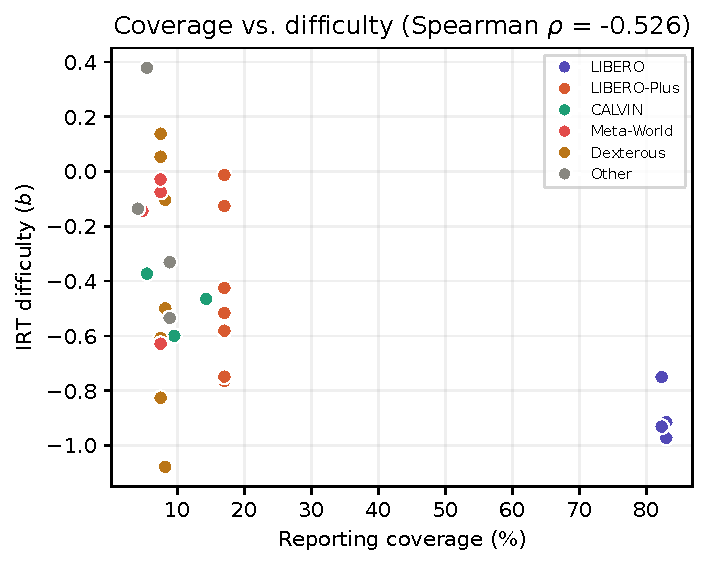
\includegraphics[width=0.58\textwidth]{figures/fig1_coverage_difficulty.pdf}
\caption{Item coverage vs.\ IRT difficulty (Spearman $\rho = -0.526$). Harder items are less reported, consistent with selection bias. Colors indicate benchmark family.}
\label{fig:covdiff}
\end{figure}

\subsection{The AD-IRT Mechanism}

The learned $w$ is consistently negative ($\bar{w} = -0.50$), meaning the MIRT weight $\alpha$ \emph{decreases} with family count. This reverses the na\"ive expectation that broad-coverage models should receive more MIRT. We offer the following explanation: MIRT's item parameters $\mathbf{a}_j$ and $d_j$, estimated from the full dataset, encode cross-family difficulty calibration. A narrow-coverage model (e.g., reporting only four LIBERO suites) benefits from this calibration because MIRT's item loadings encode the relative difficulty of LIBERO-Long versus LIBERO-Spatial---information not available to the 1PL model, which estimates $b_j$ independently. Models with broad coverage already have enough items for 1PL to estimate $\theta$ accurately, so the additional MIRT signal provides diminishing returns.

\begin{figure}[htbp]
\centering
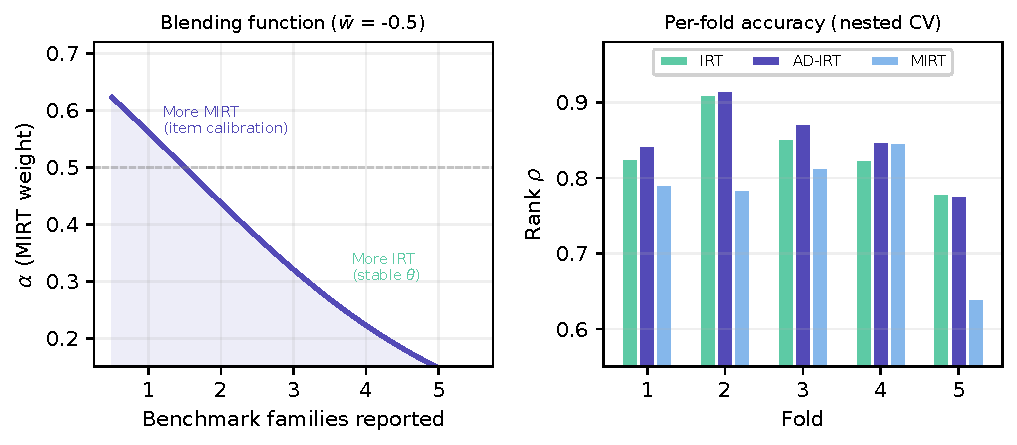
\includegraphics[width=0.95\textwidth]{figures/fig2_mechanism.pdf}
\caption{Left: AD-IRT blending function ($\bar{w} = -0.5$). MIRT weight is higher for narrow-coverage models (item-side calibration) and lower for broad-coverage models (stable IRT $\theta$). Right: Per-fold ranking accuracy comparison.}
\label{fig:mechanism}
\end{figure}

\FloatBarrier
\section{Discussion}

\paragraph{Item-side vs.\ model-side MIRT contribution.} The counterintuitive $w < 0$ finding suggests a reframing: MIRT's value in sparse evaluation is not primarily through multidimensional ability estimation (which requires broad per-model coverage) but through structured item difficulty estimation (which benefits from the full dataset). This is consistent with the LLTM perspective~\citep{fischer1973}, where item features decompose difficulty---here, MIRT's item loadings serve a similar function.

\paragraph{Connection to EFSL.} AD-IRT extends EFSL~\citep{kang2026efsl} along a second axis. EFSL showed IRT corrects ranking failures from sparsity and difficulty heterogeneity. AD-IRT shows that adaptive-complexity blending further improves over fixed-complexity IRT when item diversity varies across the model population.

\paragraph{Limitations.} (1)~Five-fold CV has inherent variance; the $p = 0.0625$ Wilcoxon test is marginal. Larger VLA evaluation ecosystems would provide more statistical power. (2)~MIRT uses gradient descent rather than MCMC; proper Bayesian estimation~\citep{reckase2009} may improve the MIRT component. (3)~Benchmark family mapping is manual; automatic family detection via item parameter clustering is future work. (4)~Results are from one evaluation ecosystem (VLA manipulation). (5)~The observation-to-parameter ratio for MIRT ($O/P = 2.3$) is below recommended thresholds; as VLA data grows, MIRT's contribution should increase.

\section{Conclusion}

AD-IRT demonstrates that IRT and MIRT are not competing methods---they are endpoints of a complexity continuum. By blending their predictions per model based on observation coverage breadth, AD-IRT achieves the best ranking accuracy ($\rho = 0.851$, nested CV) among all tested methods on real Physical AI benchmark data, outperforming IRT ($0.839$) in 4 of 5 folds. The mechanism requires a single learned parameter, adds negligible computational cost, and---contrary to na\"ive expectation---contributes primarily through item-side calibration for narrow-coverage models. As Physical AI evaluation scales, adaptive psychometric methods will become increasingly valuable.

\paragraph{Data and code.} All data is from the public Evo-SOTA.io repository~\citep{evosota2026}. The supplementary archive includes the complete parsing script, frozen score matrix, fold assignments, fold-level results, and experiment code. Repository will be made public upon preprint release.

\bibliographystyle{plainnat}
\bibliography{references}

\end{document}
